\chapter{IBM BigFix on SaaS, la progettazione}
Per la realizzazione di un prototipo di questo tipo, è necessaria un'attenta progettazione. Quella di cui andremo a parlare a breve è la fase dell'ideazione che va dall'identificazione dei requisiti funzionali, dei bisogni dell'utente, alla definizione dei parametri qualitativi che deve avere il prodotto finale, determinando scelte molto importanti dal punto di vista architetturale. Al termine di questa fase il team inizia gli sprint di development, raffinando sempre di più il modello del servizio che si vuole realizzare. Andiamo ora a vedere quali sono i primi passi che si sono mossi nella realizzazione del progetto.

\section{Interaction Design}
Non si può prescindere dal fatto ce l'interaction design sia la primissima fase da affrontare all'inizio del progetto. Se non si parte dai reali bisogni dell'utente finale, si rischia inevitabilmente di sbagliare strada e realizzare un prodotto che non avrà mai successo sul mercato. Nell'affrontare questo tipo di progettazione l'IBM ha adottato un framework sempre più diffuso nel panorama dello studio dell'usabilità, il Design Thinking.

\subsection{Design Thinking}
Empatia. E' questa la parola chiave della filosofia del Design Thinking. E' un processo creativo che ha come scopo quello di mettere al centro del progetto le necessità dell'utente. Ma proprio per meglio comprendere queste necessità è indispensabile instaurare un rapporto di empatia con gli utenti stessi. Capire i loro reali bisogni, ma anche osservarli durante la loro vita quotidiana per comprendere quelle necessità che non vengono direttamente esternate. Al tempo stesso si vogliono massimizzare le occasioni di feedback cercando di produrre il prima possibile degli output che permettano di comparare più soluzioni alternative. Aumentando per quanto possibile gli input, si riducono le probabilità di fallimento. Ma analizziamo i diversi step che accompagnano un percorso di design thinking.
\begin{figure}[h!]
	\centering
	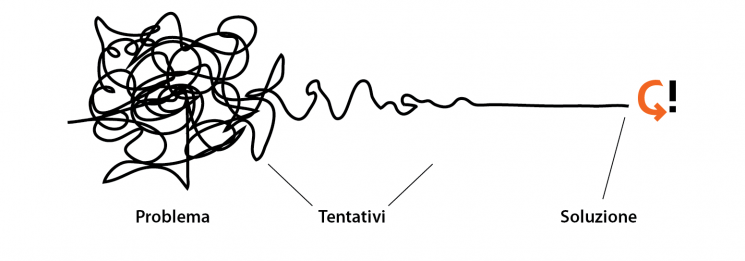
\includegraphics[width=\textwidth,keepaspectratio=true]{capitoli/imgs/Design-Thinking.png}
	\caption{Schematizzazione molto basilare del Design Thinking}
\end{figure}
\begin{itemize}
	\item Definire il problema \\
	In questa fase del lavoro è fondamentale osservare, capire le abitudini degli utenti ed immedesimarsi in loro.
	\item Divergere \\
	Qui entra in gioco la creatività, cercando di mettere sul piatto il maggior numero di soluzioni possibili, evitando però preconcetti sulle soluzioni e concentrandosi solamente sul problema.
	\item Testare \\
	E' necessario ora produrre dei prototipi testabili in modo che si possano comparare le diverse soluzioni e ricevere feedback dagli utenti.
	\item Convergere \\
	A questo punto è il tempo di dirigersi verso una soluzione, utilizzando anche la creatività per attuare dei compromessi tra quelle soluzioni parziali che intersecano al meglio i requisiti.
\end{itemize}


\subsection{BigFix SaaS Interaction Design}
Il nodo cruciale di questa fase del lavoro e stato per noi quello di capire realmente quale fosse il target del nuovo servizio SaaS e quali siano i reali bisogni che possano spingere i clienti ad adottare un prodotto SaaS, siano essi già degli utenti della versione on premise o no. Il problema principale prima dell'avvento del paradigma design thinking era che i requisiti funzionali dei prodotti che venivano realizzati per le aziende erano stabiliti tramite delle contrattazioni svolte tra i progettisti e gli addetti agli acquisti delle aziende clienti, spesso trascurando i reali beneficiari del prodotto, ossia i tecnici dell'azienda cliente. Questo spesso porta a realizzare dei prodotti che non fanno fronte ai reali bisogni dell'utente. 


\paragraph{Stakeholder Map}
L'obiettivo principale di questa fase del lavoro è stata per noi quella di allineare tutti gli interessati, sviluppatori, dirigenti e potenziali utenti, sugli obiettivi del progetto SaaS. Per fare ciò si è fatto uso della Stakeholder Map, un artefatto che raffigura per l'appunto tutti gli Stackeholder interessati alla realizzazione del progetto. 
\begin{figure}[h!]
	\centering
	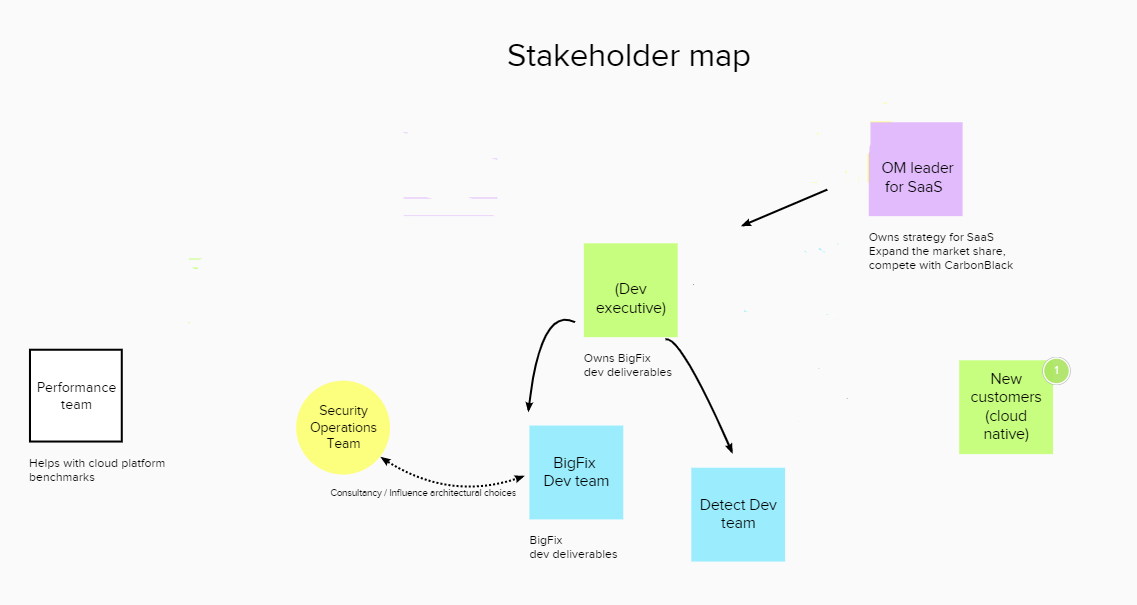
\includegraphics[width=\textwidth,keepaspectratio=true]{capitoli/imgs/StakeholderMap.PNG}
	\caption{BigFix on SaaS Stakeholder Map}
\end{figure}
Possiamo notare come gli input vengano da figure dirigenziali, che dettano le direttive aziendali, e da clienti del panorama cloud. E' inoltre necessaria una stretta interazione tra il team di sviluppo e il Security Operation Team, ovvero il team che dovrà garantire la manutenzione del servizio SaaS, monitorando le prestazioni del servizio e intervenendo se necessario.

\paragraph{User Research}
Il coinvolgimento della figura dell'utente finale è avvenuto fin dalla progettazione. Questo è stato fatto tramite interviste strutturate, ma anche osservando gli utenti nella loro routine lavorative, cercando di captare necessità e frustrazioni che vogliono essere eliminate e annotarle. L'obiettivo di fondo di questa fase del lavoro era quello di instaurare un rapporto di empatia tra gli utenti e chi realizza il progetto.

\paragraph{Nascita delle personas}
A questa punto occorreva fare un'operazione di astrazione. Cercare di identificare degli elementi chiave dal lavoro precedente e impersonare i bisogni e le caratteristiche scoperte in delle personas. Le personas sono personaggi fittizi che vengono creati per rappresentare i diversi tipi di utenti in base alle loro caratteristiche comportamentali. Vengono utilizzate per creare degli scenari e capire meglio il target del lavoro che si sta per compiere. Nel nostro caso sono state individuate le seguenti personas:
\begin{itemize}
	\item Rick - BigFix Operator \\
	Rick è l'amministratore che utilizza BigFix nella sua versione SaaS. Vuole poter gestire gli endpoint della sua azienda come farebbe con la versione on premise, distribuire contenuti e forzare le policy aziendali. usa le applications di BigFix.
	\item James - Content Creator \\
	James crea i contenuti per BigFix, crea Fixlet e task ad hoc per la propria azienda e crea pacchetti da deployare su diversi endpoint aziendali.
	\item Scott - BigFix Architect \\
	Scott è l'architetto dell'azienda cliente. Si occupa di installare la suite BigFix, che nel caso della versione SaaS risulta essere molto più agevole. Deve stabilire quale sia l'architettura azienda aziendale, relay e la rete di agent.
	\item  Rafael - Security Analyst \\
	Rafael è la figura che si occupa di controllare che gli endpoint rispettino le policy aziendali e può mandare dei messaggi per sollecitare l'attuazione della compliance.
	\item Lucy - IT Manager \\
	Si occupa della gestione dell'infrastruttura IT dell'azienda. Ha bisogno di accedere a molti contenuti dell'operator e si interfaccia spesso con Rick.
	\item Hugo - OPS engineer \\
	Hugo è un dipendente IBM che si occupa della manutenzione del servizio SaaS.
\end{itemize}

\paragraph{Empathy Map}
A questo punto è stato necessario definire gli aspetti caratteriali dal punto di vista lavorativo delle personas appena individuate. Questo si formalizza attraverso una Empathy Map per ogni peronas che si vuole analizzare. In questo artefatto vengono poste al centro e ne vengono appuntate le peculiarità. Abbiamo scritto cosa fa durante la giornata e le sue necessità, ma anche dopo un'analisi quelli che possono essere i suoi sentimenti durante lo svolgimento dei task quotidiani. tra le caratteristiche che abbiamo cercato di delineare nei personaggi ci sono:
\begin{itemize}
	\item Profilo professionale
	\item Attività
	\item Attitudini
	\item Bisogni
	\item Obiettivi
	\item Cosa possiamo fare per aiutarlo
\end{itemize}
\begin{figure} [h!]
	\centering
	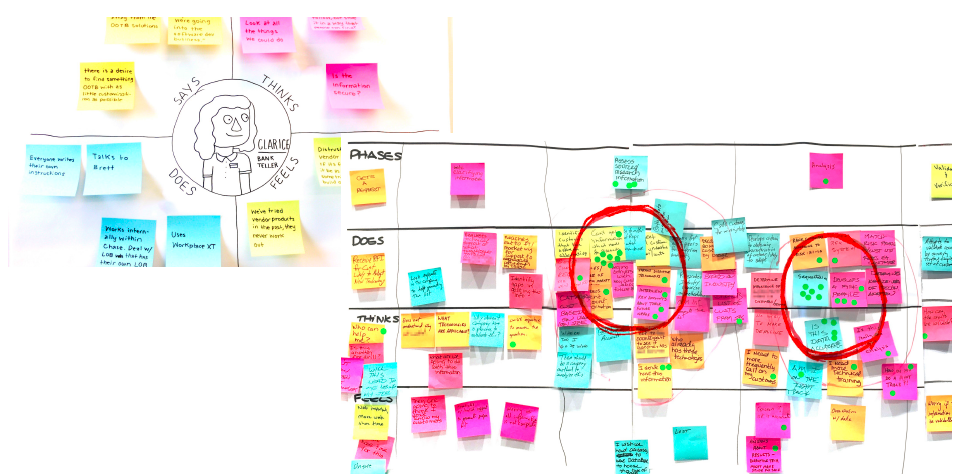
\includegraphics[width=0.7\linewidth]{capitoli/imgs/empatymap}
	\caption{Esempio di Empathy Map}
	\label{fig:empatymap}
\end{figure}
\begin{figure} [h!]
	\centering
	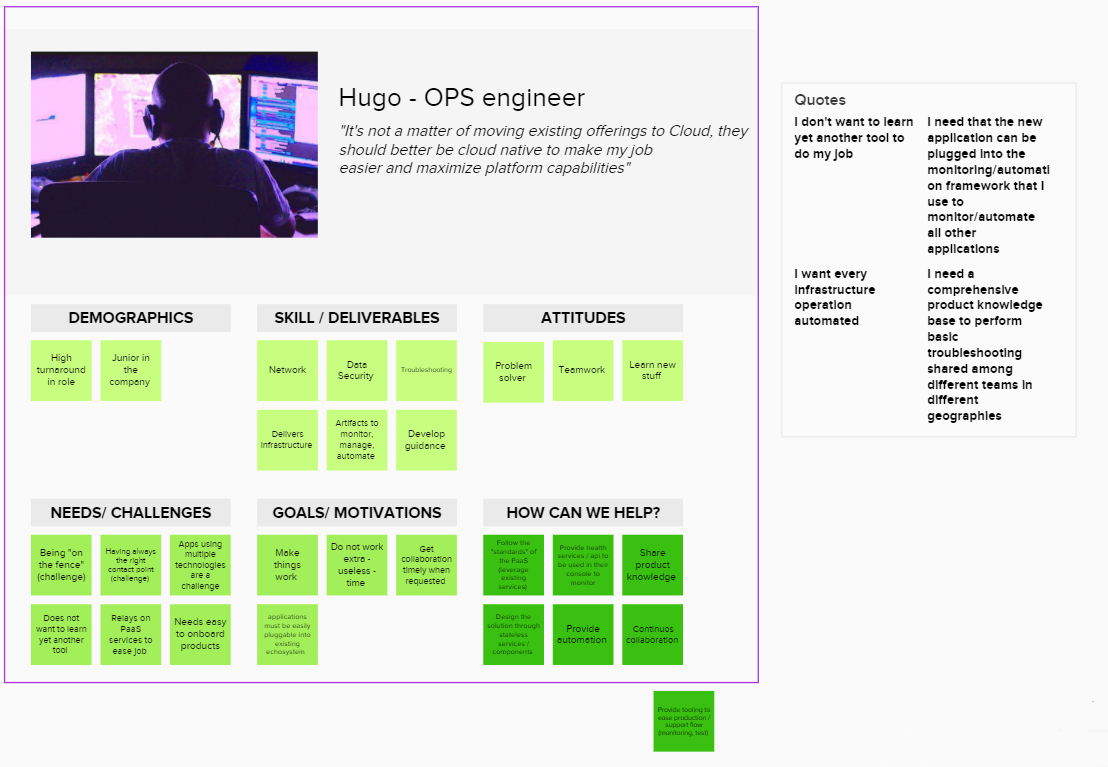
\includegraphics[width=0.7\linewidth]{capitoli/imgs/HugoEM.PNG}
	\caption{Empathy Map di una delle nostre personas}
	\label{fig:hugoem}
\end{figure}

\paragraph{Scenario Map}
In questo nuovo elaborato le personas con le quali siamo entrati in confidenza nella fase precedente iniziano ad essere inserite nel loro ciclo di vita quotidiano. Con lo scenario viene descritto un flusso di lavoro tipico del personaggio in questione. Nel succedersi degli stages, ovvero i passi in cui si divide lo scenario, si annotano quelli che possono essere i sentimenti dell'utente, cercando di individuare gli elementi di frustrazione e le opportunità per intervenire nella progettazione risolvendo i problemi dell'utente tipo. Vediamo qui di seguito una scenario map per Rafael.
\begin{figure} [h!]
	\centering
	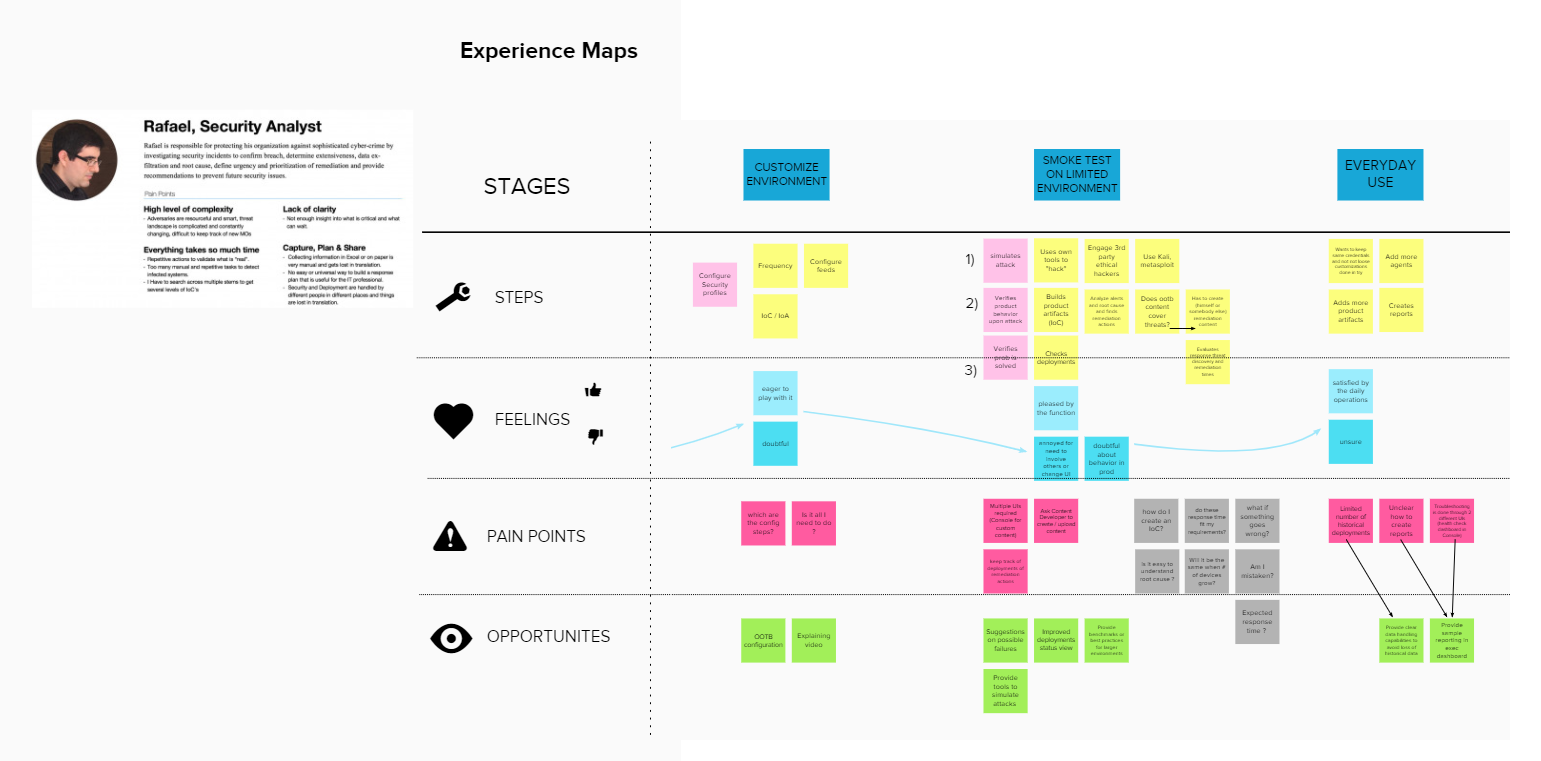
\includegraphics[width=0.7\linewidth]{capitoli/imgs/scenarioRafael.PNG}
	\caption{Scenario che rappresenta il primo utilizzo del servizio da parte di Rafael, il Security Analist }
	\label{fig:scen1}
\end{figure}

\paragraph{}
Vediamo qui di seguito uno schizzo riassuntivo degli step del Design Thinking che abbiamo adottato:
\begin{figure} [h!]
	\centering
	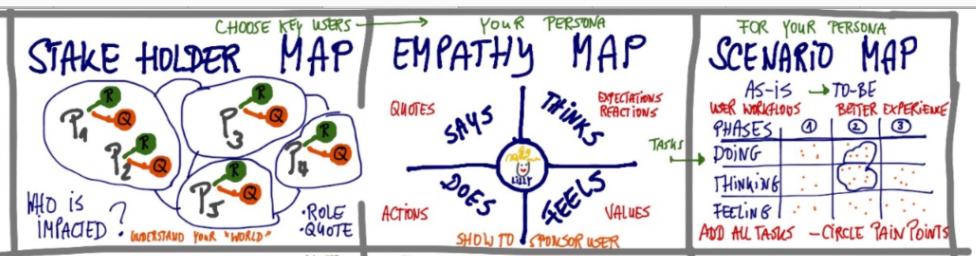
\includegraphics[width=0.7\linewidth]{capitoli/imgs/schizzodesthink.PNG}
	\caption{Step del Design Thinking adottati nel nostro progetto}
	\label{fig:dt}
\end{figure}

\paragraph{}
Gli scenari in questo modo individuato vanno a rappresentare la base per la stesura delle Epiche. Queste, come abbiamo descritto nella sezione 2.3 verranno poi raffinate con la stesura delle Storie e infine divide nei Task implementabili dagli sviluppatori.
\begin{figure} [h!]
	\centering
	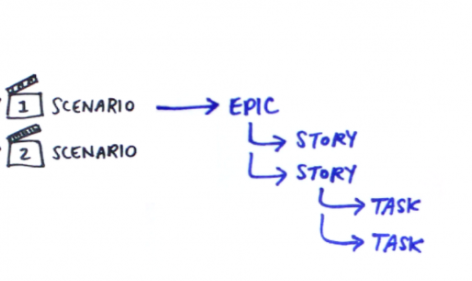
\includegraphics[width=0.7\linewidth]{capitoli/imgs/scenario.PNG}
	\caption{Relazione tra gli scenari individuati in questa fase e le Epiche del framework SCRUM}
	\label{fig:scentospic}
\end{figure}

\section{Requisiti Non Funzionali}
Abbiamo già parlato nel capitolo 4 di quali sono le nuove problematiche alle quali una SaaS application deve far fronte. Ovviamente nel mio lavoro di tesi questo aspetto è stato un argomento cruciale delle prime fasi del lavoro. Soddisfare questo tipo di requisiti comporta infatti fare scelte architetturali molto impattanti e in quanto tali occorre definirle prima possibile nel design di un sistema software. 

\subsection{Dependability}
Il servizio di BigFix SaaS è stato progettato per garantire, quando sarà in produzione, un'availability che si mantenga sempre su valori superiori al 99. Ovviamente si prevedono carichi di utilizzo che possono essere anche molto elevati. La suite di BigFix è utilizzata contemporaneamente da clienti di tutto il mondo, alcuni dei quali possiedono una rete di endpoint composta da un numero considerevole di nodi. Tutto ciò può portare a picchi di carico molto elevati nonostante i quali il servizio deve continuare a essere disponibile con prestazioni sopra delle soglie minime di accettabilità.

\paragraph{Microservizi e container}
Come abbiamo potuto osservare nei capitoli precedenti, l'adozione di microservizi e container è un must per i servizi cloud. Grazie a questa scelta possiamo garantire agli utenti di BigFix SaaS un'alta Dependability, fattore fondamentale nel contesto della security aziendale in cui si va a calare questa suite di prodotti. I microservizi di BigFix, infatti, verranno replicati tramite i container in data center IBM in tutto il mondo, ciò potrà garantire anche tolleranza ai guasti che possono presentarsi. Il grado di replicazione dei diversi microservizi sarà ovviamente proporzionale all'importanza del microservizio stesso. Ci saranno ovviamente dei microservizi con dei ruoli più centrali di altri.

\subsubsection{Rolling Update}
Un'altro aspetto critico nel garantire un'alta availability è quello dell'aggiornamento del servizio. Facendo un paragone con i servizi SaaS che utilizziamo quotidianamente per consultare la posta elettronica, notiamo che non assistiamo mai a fenomeni di mancanza del servizio quando il prodotto si aggiorna, ma, all'occorrenza, troviamo già il prodotto nella sua versione aggiornata. Vogliamo che questo comportamento si verifichi anche con la suite SaaS di BigFix e per questo occorre attuare una politica di Rolling Update. Silentemente, vengono aggiornate a turno tutte le repliche dei microservizi interessanti dall'aggiornamento. Nel fare ciò però, l'esperienza utente non risente di peggioramenti, in quanto le repliche che rimangono in servizio garantiscono l'efficienza del servizio.

\subsubsection{Utilizzo di DB2}
Anche la persistenza dei dati può risultare essere un elemento critico per la dependability. Occorre uno strumento che garantisca l'integrità dei dati, la resistenza ai guasti con adeguate misure di ripristino e soprattutto la riservatezza dei dati che, in un contesto come la security aziendale, possono essere molto sensibili. Si è scelto di utilizzare come DBMS DB2, un database relazionale prodotto da IBM. Una peculiarità di questo prodotto è la HADR (High Availability and Disaster Recovery). Diamo un'occhiata all'architettura di DB2 per capire di cosa si tratta.

\begin{figure}[h!]
	\centering
	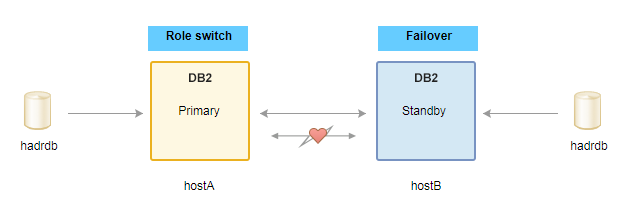
\includegraphics[width=\textwidth,keepaspectratio=true]{capitoli/imgs/db2.PNG}
	\caption{Architettura del DBMS IBM DB2}
\end{figure}

\paragraph{}
DB2 replica tutto il contenuto del suo database, chiamato Primary Database, in un secondo database detto Standby Database, il quale svolge anche il ruolo di backup. I dati di questi due sono consistenti e vengono sincronizzati costantemente. Qualunque malfunzionamento del database principale normalmente comporterebbe dei tempi di non availability più o meno lunghi. Con questa architettura HADR, invece, nel momento in cui il Primary Database presenta un guasto, lo Standby Database assume il suo ruolo (Failover) finché il database primario non torna disponibile e, a qual punto, i due database tornano a svolgere il loro compito originario (Role switch). Una prerogativa importante però è che i due database risiedano in due data center distinti, o comunque provengano da due fonti di energia distinte nel caso si trovino nello stesso luogo geografico, per evitare che dei guasti possano colpirli entrambi. 

\subsection{Scalabilità}
Per quanto riguarda la Scalabilità ci prefiggiamo di garantire le stesse specifiche del prodotto in versione on premise, quindi di supportare fino a 250.000 endpoint per server. Il soddisfacimento di questa specifica, nel contesto SaaS, sposta l'attenzione ovviamente sul nuovo concetto di server, ossia una serie di microservizi distribuiti che svolgono le funzionalità che nella versione on premise era svolta dal server presso il client. Ancora una volta sta nella ridondanza dei microservizi la chiave per garantire la scalabilità prefissata.

\subsection{Monitoring}
Sotto l'aspetto del monitoring ci siamo dovuti scontrare con una nuova complessità nel saper monitorare un servizio così diffuso come quello di SaaS. La necessità è quella di sostituire l'intervento umano nella consultazione dei log di tutti i servizi. Il requisito che abbiamo è quello di analizzare i risultati, saper effettuare delle medie e calcolare dei picchi di parametri come il throughput o la latenza. Vogliamo infine che questa mole di dati fosse facilmente consultabile agli occhi di chi effettua la manutenzione del prodotto, magari sotto forma di grafici facilmente intellegibili. Per soddisfare queste necessità abbiamo individuato i tool Prometheus e Grafana che si sono rivelati molto utili nelle fasi successive al deployment, come vedremo in seguito.  


\section{Gap con il prodotto on premise}
La natura di un servizio SaaS porta con se alcune differenze strutturali importanti con il prodotto già esistente. La modalità di fruizione del prodotto è completamente diversa dal prodotto on premise infatti e gli accorgimenti sono da prendere subito in considerazione in quanto impattano pesantemente sulle scelte architetturali.
\paragraph{Introduzione della multitenancy}
Uno di questi è sicuramente la multitenancy. Nel modello SaaS può capitare che sulla stessa macchina fisica risiedano più server di clienti diversi. Dalla prospettiva utente però si deve dare l'impressione di un possesso esclusivo del server tramite strategie di multitenancy. E' di fondamentale importanza che un cliente non entri in contatto con dati afferenti al server di altre organizzazioni, anche se queste risiedono sullo stesso server fisico. Tra gli accorgimenti attuati c'è la modifica della modalità di archiviazione dei dati, permettendo di filtrare i dati appartenenti al tenant corretto e speciali privilegi di utilizzo dei servizi server. 
\paragraph{Introduzione dei microservizi}
L'introduzione dei microservizi è un elemento centrale della conversione a SaaS. Per attuarla è necessario un attento percorso di refactoring del codice del prodotto, suddividendolo in servizi coesi che possano rappresentare delle entità separate che cooperino tra loro.

\section{Scelta dei tool e dei servizi da utilizzare}
Nel mio caso mi sono mosso in un ambito, quello del cloud computing, si privo di una consolidata storia alle spalle, ma anche ricco di continui nuovi contributi. Infatti compaiono sempre nuove tecnologie dedicate esclusivamente all'ambiente cloud, molte delle quali open-source con frequentissimi contributi da parte degli sviluppatori.

\paragraph{}
Trattandosi della realizzazione di un prototipo SaaS, l'attenzione principale non poteva che ricadere sui container e sui più diffusi trend in ambito cloud. Si è scelto di adottare l'utilizzo dei container. Come largamente trattato nella sezione 5.2 essi rappresentano una tecnologia fondamentale per realizzare un servizio SaaS. Avendo scelto di adottare i container occorreva quindi scegliere una piattaforma che automatizzi il deployment dei container in maniera efficace. Da questo punto di vista la scelta è ricaduta su Docker, una scelta quasi obbligata vista l'alta competitività del tool e l'affermazione ormai incontrastata. In questo modo ci si alleggerisce dall'overhead di utilizzare un'intera macchina virtuale per ogni container in quanto tutti i container sulla stessa macchina fisica condividono lo stesso sistema operativo, ma al tempo stesso sono isolati. 

\paragraph{}
A questo punto però bisogna immaginare uno scenario in cui il servizio che sono andato a realizzare e scomposto in un numero piuttosto elevato di container, alcuni andranno creati in delle situazioni specifiche, altri eliminati o modificati. Per queste funzionalità l'IBM ha come direttiva quella di utilizzare Kubernetes, del quale abbiamo parlato anche nella sezione 5.2. Tramite questo tool sono in grado di orchestrare i container e controllarne il flusso di vita tramite i pod.

\section{Definizione Architetturale}
La definizione di un'architettura di un prodotto così complesso è guidata da un'attenta analisi dei requisiti appena descritti. Occorre stabilire quali siano i componenti da implementare, altri da riutilizzare e alcuni da adattare. Inoltre occorre stabilire come interfacciarsi con nuove tecnologie che devono essere opportunamente inserite nel contesto di applicazione.

\subsection{Viste architetturali}
\subsubsection{Vista sull'architettura fisica e sui container}
\begin{figure} [h!]
	\centering
	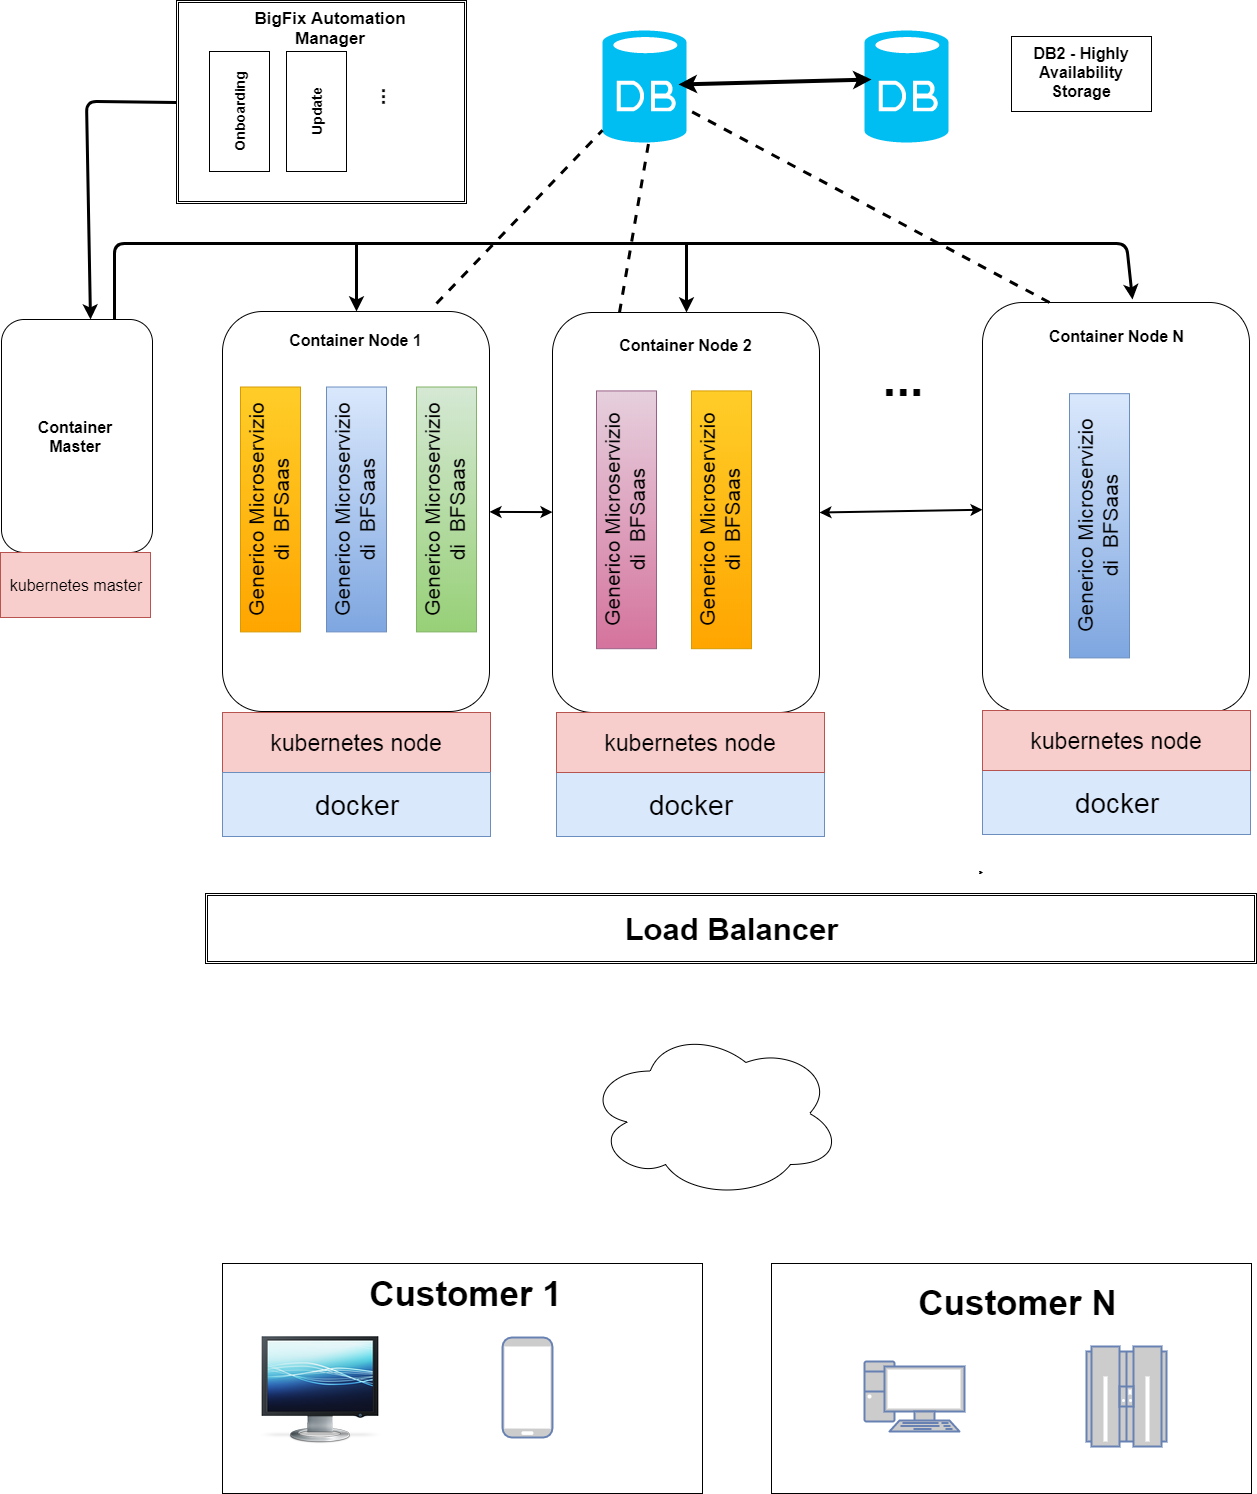
\includegraphics[width=1\linewidth]{capitoli/imgs/BfsaasArchitecture.png}
	\caption{Architettura di BigFix SaaS}
	\label{fig:arch}
\end{figure}
Questa è la più significativa delle viste architetturali. Da questa immagine possiamo chiaramente evincere la struttura a microservizi del SaaS di BigFix. Ogni microservizio è deployato in un container. Volutamente non si sono volute raffigurare macchine che ospitano i container per rendere il senso di portabilità dei container stessi. Potrebbero trovarsi tutti sulla stessa macchina fisica come in parti del mondo differenti. Tutti i container, come abbiamo sottolineato precedentemente, adottano Docker come gestore. Da questa architettura notiamo anche la presenza di nuovi componenti:
\begin{itemize}
	\item Container Master \\
	Questo container ospita il componente Kubernetes master, il quale ha il compito di governare il comportamento di tutti gli altri nodi container. Questi ultimi rappresentano infatti dei Kubernetes node.
	\item BigFix Automation Manager \\
	Questo componente è fondamentale per tutti i processi di gestione, che vedremo in seguito. SI immagino ad esempio scenari come l'onboarding di un nuovo cliente o la distribuzione di una versione del servizio.
	\item Load Balancer \\
	Come suggerisce il nome stesso è il componente che ha la responsabilità di ripartire il carico di lavoro sui microservizi presenti sui container, alcuni di loro replicati. Una buona gestione del workload è fondamentale nelle situazioni di picco di utilizzo da parte dei clienti per garantire l'availability del prodotto.
\end{itemize}

\subsubsection{Viewpoint dell'utente utilizzatore}
\begin{figure} [h!]
	\centering
	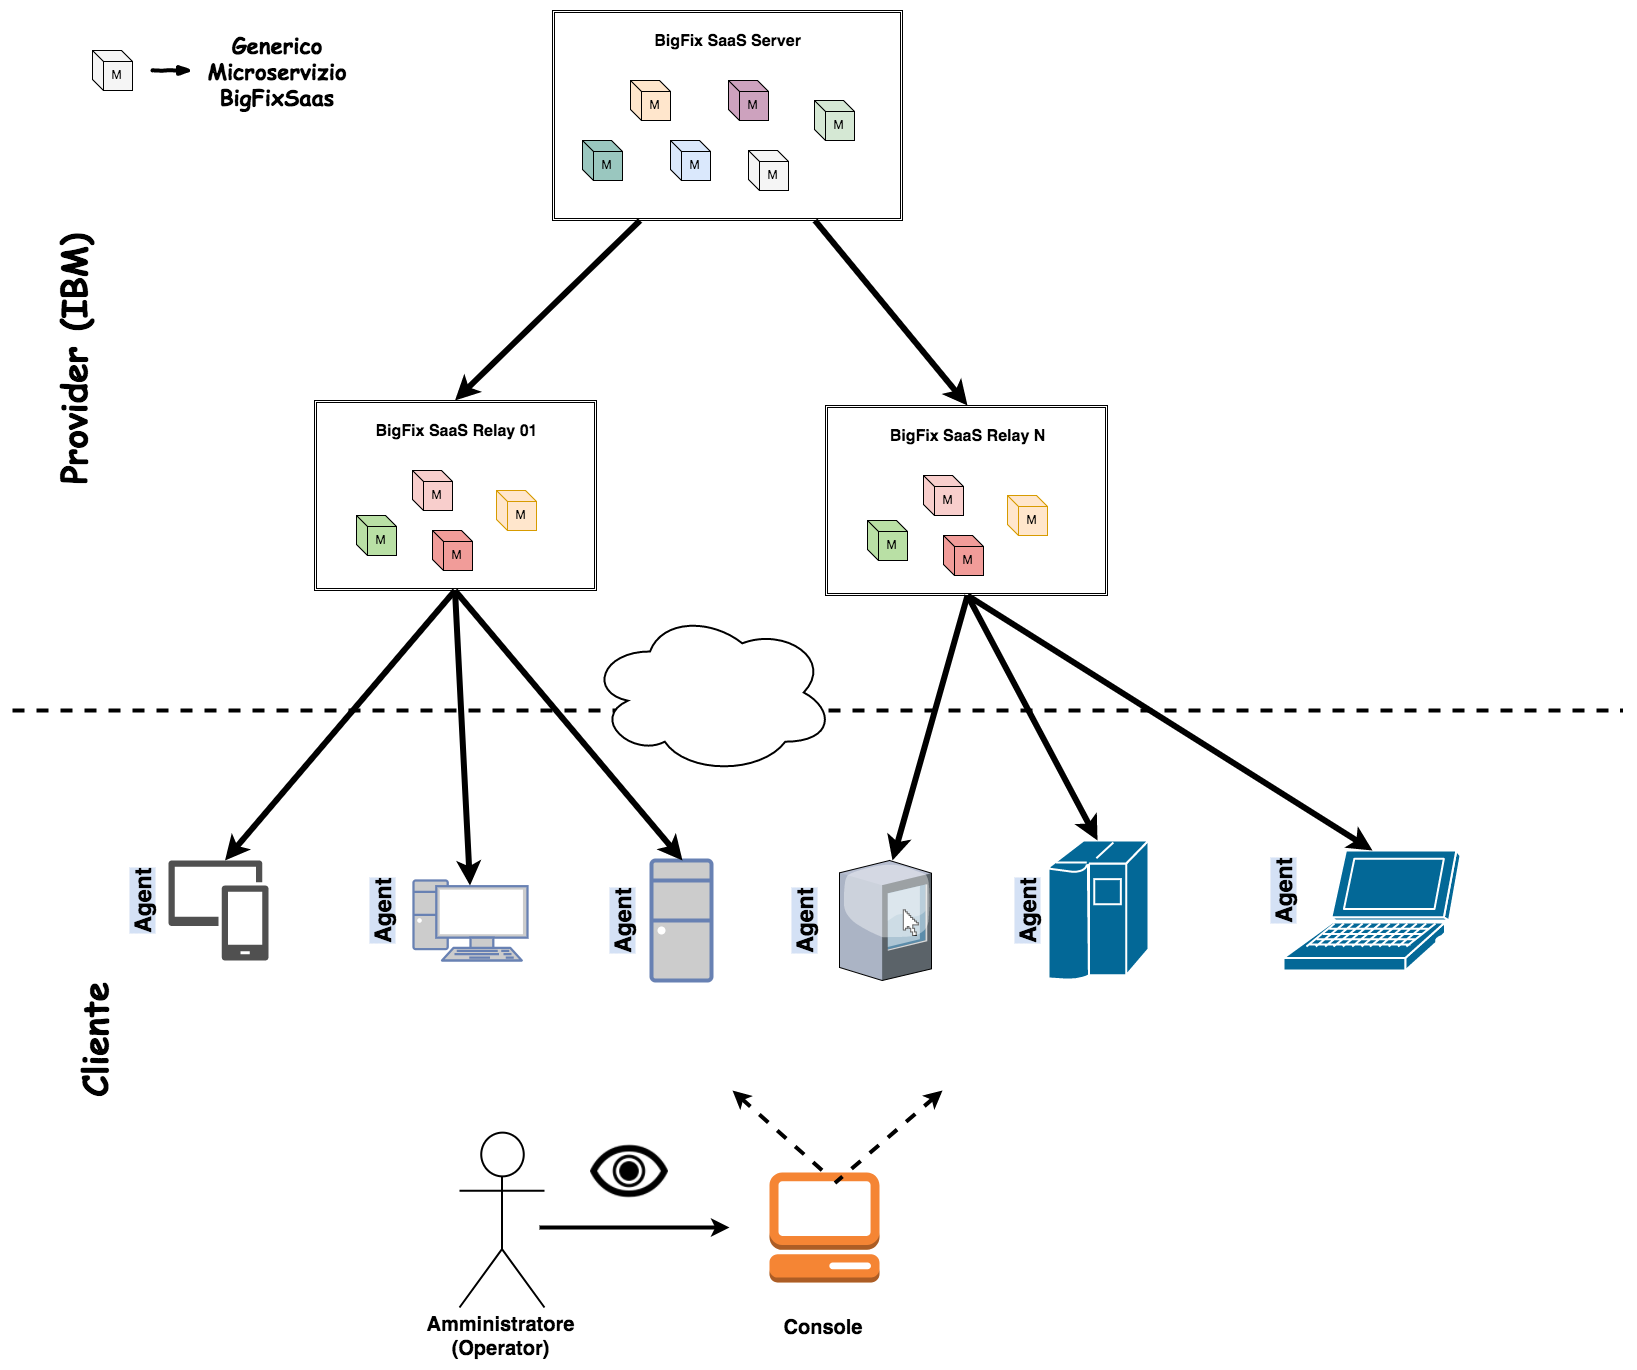
\includegraphics[width=1\linewidth]{capitoli/imgs/architectureUserViewpoint.png}
	\caption{Architettura di BigFix SaaS}
	\label{fig:uviewpoint}
\end{figure}
Da questa immagine invece cerchiamo di ricostruire la struttura tradizionale di BigFix rivisitandola però in ottica SaaS. Le componenti del server e dei relay non sono più macchine fisiche facenti parte dell'infrastruttura del cliente. Il server e il relay sono completamente sotto il controllo del provider e sono composti da opportuni microservizi che cooperano per garantire le funzionalità del servizio. L'unico componente che rimane fisicamente dal cliente è l'agent, che è presente ovviamente in ogni dispositivo della rete di endpoint.

\section{Definizione dei processi di gestione}
Una delle novità nel distribuire un servizio SaaS riguarda i processi di gestione. Analogamente alla progettazione architetturale, anche i processi di gestione vanno ben definiti e, successivamente, messi in opera.

\subsection{Novità rispetto al prodotto già esistente}

\paragraph{Onboarding}
Si pensi ad esempio allo scenario dell'onboarding di  un nuovo cliente. Il sistema deve garantire che un processo completamente automatico possa portare il nuovo utente dal click sulla form di registrazione a tutto il servizio BigFix pronto all'utilizzo in pochi minuti, al massimo ore. Gli utilizzi del servizio hanno delle dinamiche molto diverse rispetto allo scenario on premise.

\paragraph{Monitoring}
Anche il monitoring delle attività e delle prestazioni richiede nuovi strumenti perché sposta l'attenzione sull'utilizzo dei container e sul funzionamento dei microservizi. Abbiamo definito dei processi specifici (Prometheus) che sappiano monitorare i pod di Kubernetes e, conseguentemente, i container.

\subsection{Disaster Recovering}
Dal punto di vista del disaster recovery con un servizio SaaS abbiamo notevolmente diminuito il rischio di verificarsi di situazioni di criticità, in quanto le infrastrutture fornite dal provider sono molto più efficienti da questo punto di vista. Al tempo stesso però, nel caso del verificarsi di qualche malfunzionamento il pericolo è notevolmente maggiore. A quel punto infatti potrebbero essere coinvolti tutti i clienti forniti dal servizio. In uno scenario del genere abbiamo progettato misure di emergenza che prevedono a redistribuzione del carico tra i microservizi ma anche l'attuazione del recovery di emergenza di db2.
